\documentclass{article}
\usepackage{graphicx} % Required for inserting images
\usepackage[utf8]{inputenc}
\usepackage{hyperref}
\usepackage[letterpaper, portrait, margin=1in]{geometry}
\usepackage{enumitem}
\usepackage{amsmath}
\usepackage{booktabs}
\usepackage{graphicx}
\usepackage{float}
\usepackage{hyperref}
\usepackage[flushleft]{threeparttable}
\usepackage{textcomp}
\hypersetup{
colorlinks=true,
    linkcolor=black,
    filecolor=black,      
    urlcolor=blue,
    citecolor=black,
}



\usepackage{titlesec}
  
\title{Homework 2 Submission}
\author{David Wilson \\ Economics 7103}
\date{\today}

  
\begin{document}
  
\maketitle

\section*{Introduction}

For this assignment we were given access to imaginary data on a energy-efficiency retrofit program in Atlanta and asked to analyze if the program reduced energy usage. Houses were assigned to either a treatment or control group where the treatment group received the retrofit and the control group did not.

\section{Python}
    \subsection{Balance Table} 
    To analyze the randomization of the treatment and control groups we need to create a balance table. Table 1 below shows the sample mean and standard deviation between the treatment and control groups.\

\begin{table}[h]
    \centering
    \begin{threeparttable}
    \caption{Balance Table from Python}
        \begin{tabular}{lccc}
\toprule
 & Control & Treatment & P-value \\
\midrule
Monthly electricity consumption (kWh) & 1181.33 & 1086.75 & 0.001 \\
  & (454.31) & (423.96) & [3.403] \\
Size of home in ft^2 & 1633.05 & 1657.55 & 0.572 \\
  & (682.90) & (686.27) & [-0.566] \\
Average outdoor temperature in F\textdegree & 79.89 & 79.89 & 0.987 \\
  & (2.16) & (1.97) & [-0.016] \\
Observations & 501 & 499 &   \\
\bottomrule
\end{tabular}

        \begin{tablenotes}
          \small \item \textbf{Note:} Columns 1 and 2 contain the mean and standard deviations for each variable in the control and treatment groups. Column 3 has the P-value for the difference in means tests with the t-statistic in parenthesis.  
        \end{tablenotes}
    \end{threeparttable}
\end{table}

The balance table shows that there is not enough difference between the two groups that would be evidence of selection bias. 

\subsection{Graphical Evidence}

Figure 1 below shows the density plot of both treatment and control group. The fact that the retrofitting consumes less electricity at all levels shows that the retrofitting has worked.

\begin{figure}[H]\centering
    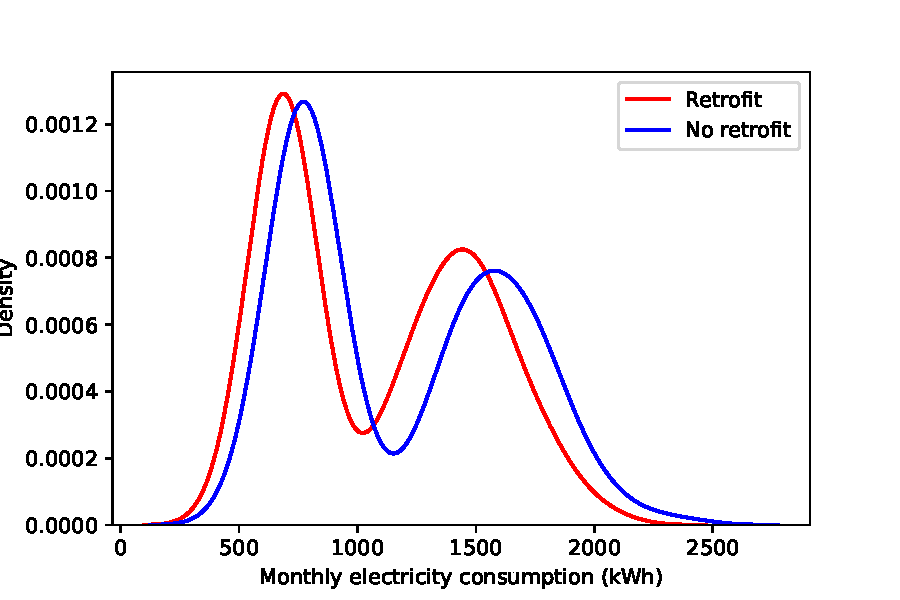
\includegraphics[width=0.7\linewidth]{kdensity.pdf}
    \caption{Density plot of electricity consumption}
\end{figure}

\subsection{OLS}

\begin{table}[h]
    \centering
    \begin{threeparttable}
    \caption{OLS Estimates Using Different Methods}
        \begin{tabular}{lccc}
\toprule
 & By Hand & Stats Model & Least Squares \\
\midrule
Received retrofit & -109.666 & -109.666 & -109.666 \\
  & (7.948) & (7.948) & (7.948) \\
Size of home in ft^2 & 0.615 & 0.615 & 0.615 \\
  & (0.006) & (0.006) & (0.006) \\
Average outdoor temperature in F\textdegree & 3.255 & 3.255 & 3.254 \\
  & (1.924) & (1.924) & (1.924) \\
Constant & -83.603 & -83.603 & -83.543 \\
  & (154.360) & (154.360) & (154.360) \\
M.S.E. & 125.652 & 125.652 & 125.652 \\
\bottomrule
\end{tabular}

        \begin{tablenotes}
          \small \item \textbf{Note:} Standard errors in parentheses. 
        \end{tablenotes}
    \end{threeparttable}
\end{table}

\begin{table}[h]
    \centering
    \begin{threeparttable}
    \caption{OLS Estimates Using Different Methods with Robust Standard Errors}
        \begin{tabular}{lccc}
\toprule
 & By Hand & Stats Model & Least Squares \\
\midrule
=1 if house received retrofit & -109.666 & -109.666 & -109.666 \\
  & (7.943) & (7.943) & (7.943) \\
Square feet of home & 0.615 & 0.615 & 0.615 \\
  & (0.007) & (0.007) & (0.007) \\
Outdoor average temperature (\textdegree F) & 3.255 & 3.255 & 3.255 \\
  & (1.932) & (1.932) & (1.932) \\
Constant & -83.603 & -83.603 & -83.608 \\
  & (154.695) & (154.695) & (154.695) \\
MSE & 125.652 & 125.652 & 125.652 \\
\bottomrule
\end{tabular}

        \begin{tablenotes}
          \small \item \textbf{Note:} Robust standard errors in parentheses. 
        \end{tablenotes}
    \end{threeparttable}
\end{table}

\section{Stata}
\subsection{Balance Table}
Similarly to the previous section's Python balance table, this table has the mean for each variable of the control and treatment sample groups with their standard deviations in parentheses. It shows the exact same values as the Python version highlighting the lesson that the outcome of this procedure is the same even when using different statistical software.
\begin{table}[ht]
    \centering
    \begin{threeparttable}
    \caption{Balance Table in Stata}
        {
\def\sym#1{\ifmmode^{#1}\else\(^{#1}\)\fi}
\begin{tabular}{l*{3}{c}}
\hline\hline
                    &\multicolumn{1}{c}{Control}&\multicolumn{1}{c}{Treatment}&\multicolumn{1}{c}{P-value}\\
\hline
Monthly kWh used by the household&    1181.33 &    1086.75 &       0.001\\
                    &   (454.31) &   (423.96) &     [3.404]\\
Square footage of home&    1633.05 &    1657.55 &       0.572\\
                    &   (682.90) &   (686.27) &    [-0.566]\\
Average monthly outdoor temperature in F\textdegree&      79.89 &      79.89 &       0.987\\
                    &     (2.16) &     (1.97) &    [-0.016]\\
\hline
Observations        &         501&         499&       1,000\\
\hline\hline
\end{tabular}
}

        \begin{tablenotes}
          \small \item \textbf{Note:} Values are the mean within each sample for each variable with the standard deviations in parentheses. 
        \end{tablenotes}
    \end{threeparttable}
\end{table}

\subsection{Scatterplot}

This is a scatterplot created in Stata with the monthly energy consumption on the y-axis and the square footage of the home on the x-axis.
\begin{figure}[H]\centering
    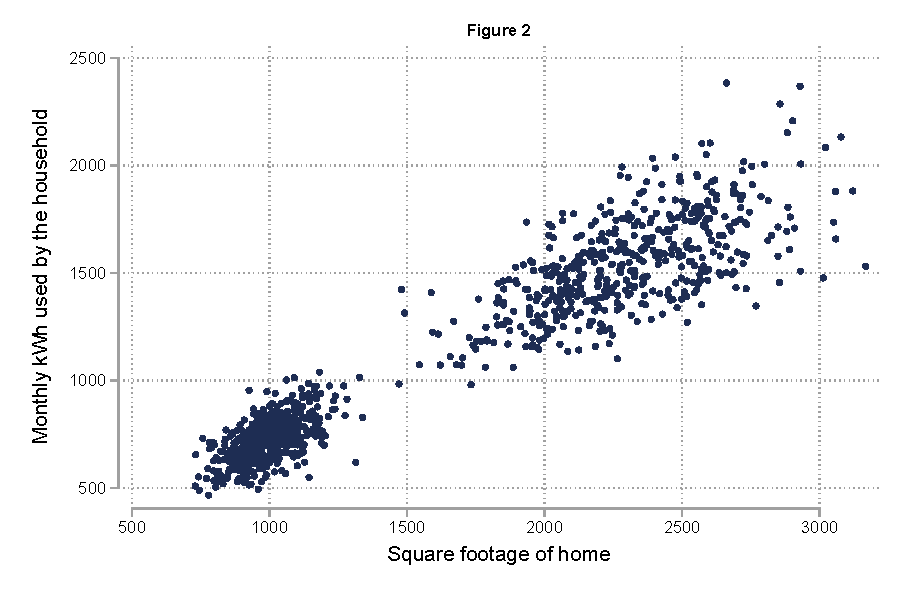
\includegraphics[width=0.75\linewidth]{twoway.pdf}
    \caption{Scatter plot showing the relationship between monthly energy consumption and the f$^2$ of a home.}
\end{figure}

\subsection{OLS regression}

Table 5 contains the OLS estimates using the Stata software. The estimate values are the same again as the ones that we received from Python.\
\\
\begin{table}[ht]
    \centering
    \begin{threeparttable}
    \caption{OLS Estimates with Robust Standard Errors}
        \begin{tabular}{l*{1}{c}}
\hline\hline
                    &\multicolumn{1}{c}{OLS}\\
\hline
Retrofitting dummy variable&    -109.666\\
                    &     (7.943)\\
Square footage of home&       0.615\\
                    &     (0.007)\\
Average monthly outdoor temperature in F\textdegree&       3.255\\
                    &     (1.932)\\
Constant            &     -83.603\\
                    &   (154.695)\\
\hline
MSE                 &     125.652\\
\hline\hline
\end{tabular}

        \begin{tablenotes}
          \small \item \textbf{Note:} Robust standard errors in parentheses. 
        \end{tablenotes}
    \end{threeparttable}
\end{table}


\end{document}